\documentclass{article}
% Chinese
% \documentclass[UTF8, nofonts, mathptmx, 12pt, onecolumn]{article}
% \usepackage{xeCJK}
% \setCJKmainfont{SimSun}
\usepackage{amsmath}
\usepackage{amsfonts}
\usepackage{amssymb}
\usepackage{wasysym}
% \usepackage{ctex}
\usepackage{graphicx}
\usepackage{float}
\usepackage{geometry}
\geometry{a4paper,scale=0.8}
\usepackage{caption}
\usepackage{subcaption}
% \newcommand{\oiint}{\mathop{{\int\!\!\!\!\!\int}\mkern-21mu \bigcirc} {}}
\newcommand*{\dif}{\mathop{}\!\mathrm{d}}
\newcommand*{\md}{\mathop{}\!\mathrm{d}}
\newcommand*{\me}{\mathrm{e}}

% \usepackage{parskip}
% \setlength{\parindent}{0cm}

\usepackage{bm}
\let\Oldmathbf\mathbf
\renewcommand{\mathbf}[1]{\boldsymbol{\Oldmathbf{#1}}}
\let\eqnarray\align

\author{Xiping Hu}
\usepackage{authblk}
\author{Xiping Hu}
\affil{https://hxp.plus/}
\title{Homework for Chapter 6}

\begin{document}
\maketitle

\begin{figure}[H]
  \centering
  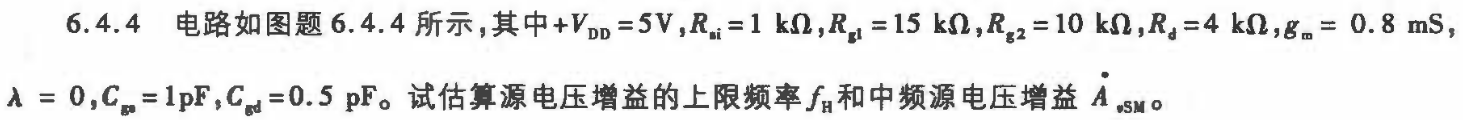
\includegraphics[width=\linewidth]{figures/Problem644}
  \label{fig:}
\end{figure}

\begin{figure}[H]
  \centering
  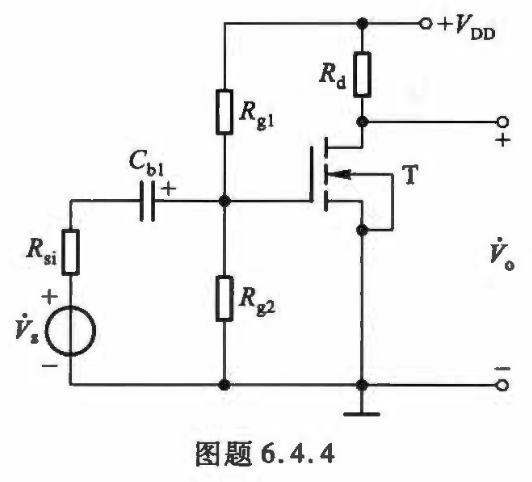
\includegraphics[width=0.4\linewidth]{figures/Problem6441}
  \label{fig:}
\end{figure}

\begin{figure}[H]
  \centering
  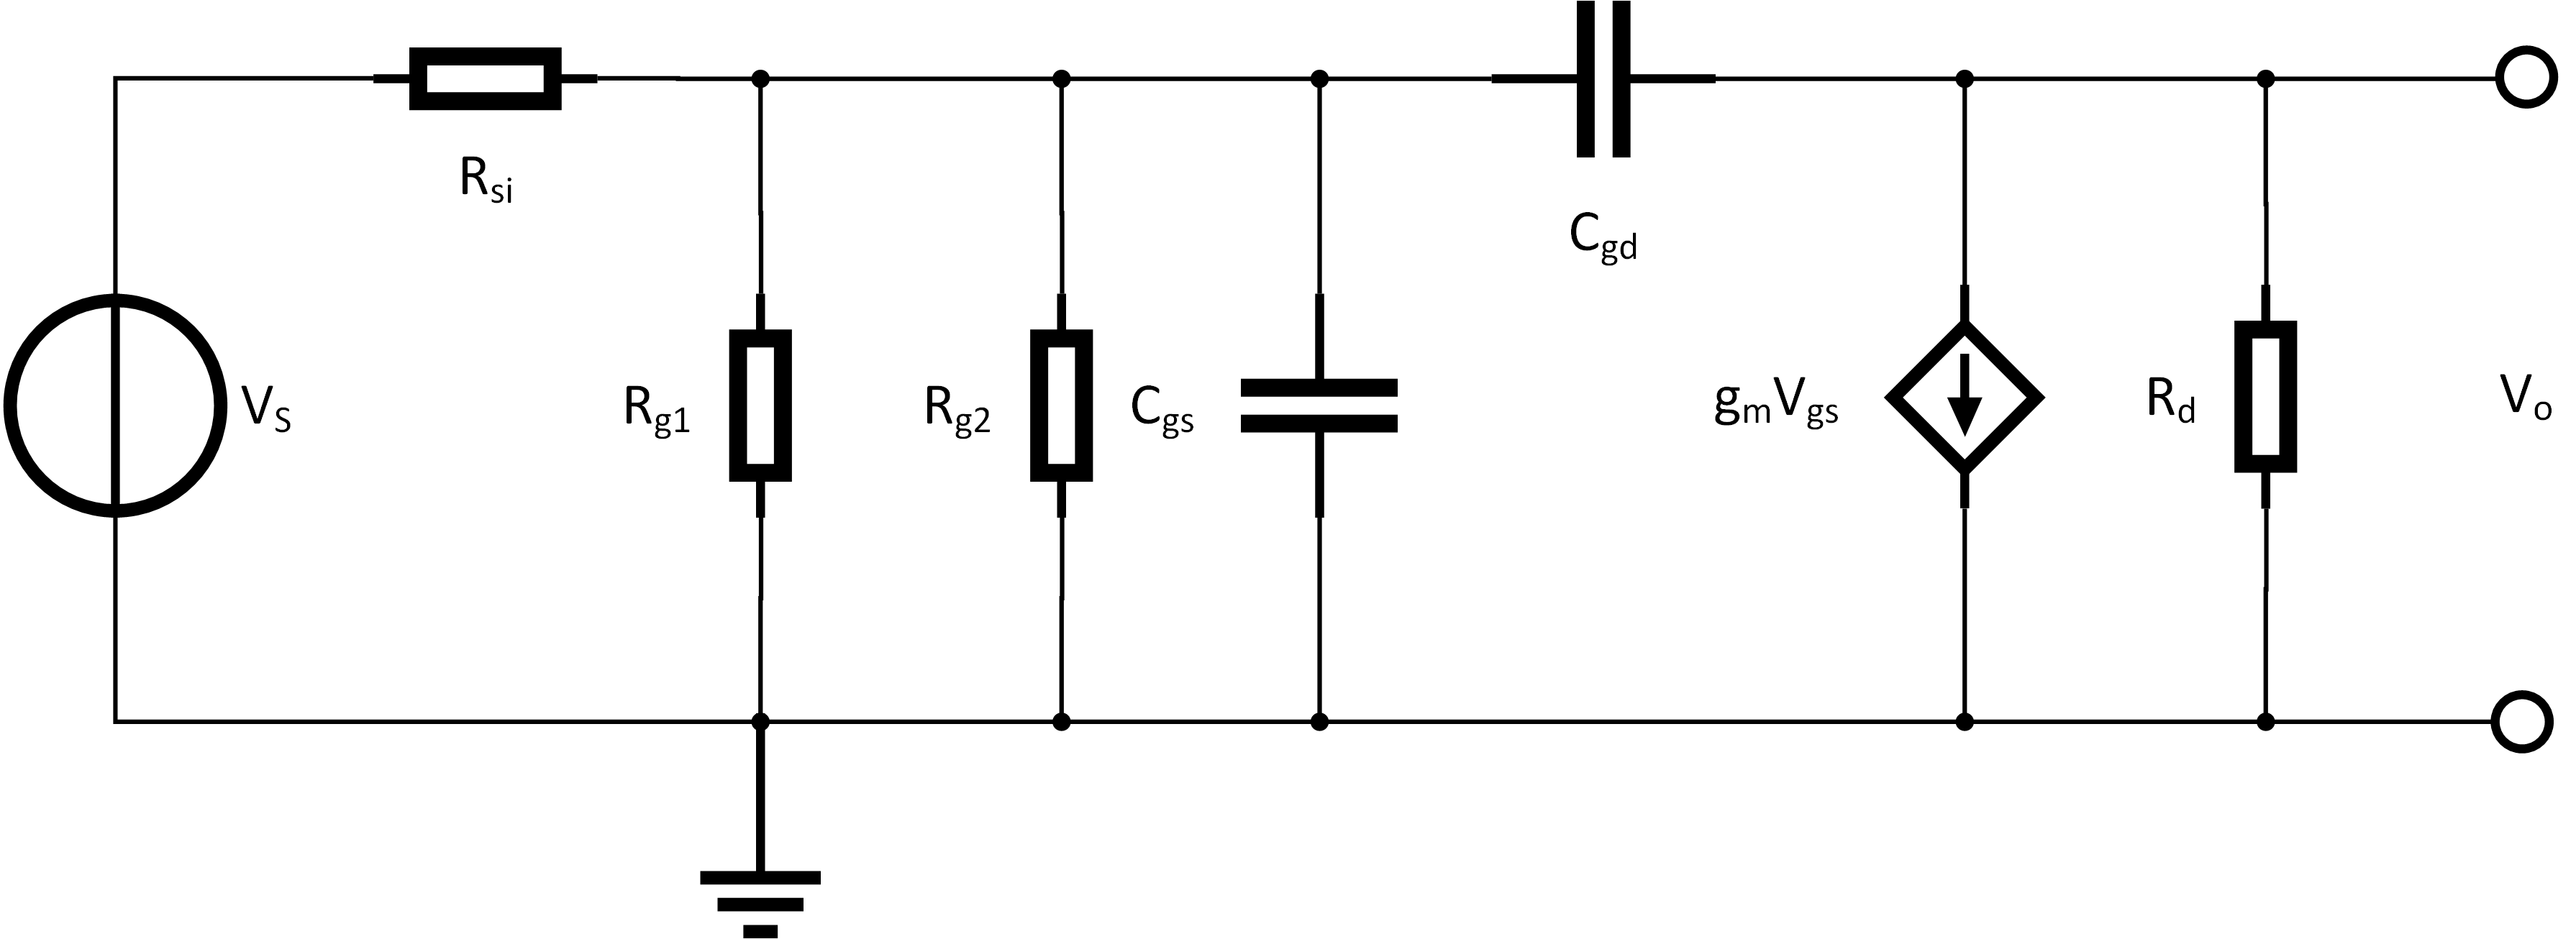
\includegraphics[width=0.5\linewidth]{figures/Problem6442}
  \label{fig:}
\end{figure}

\begin{figure}[H]
  \centering
  \begin{subfigure}{.65\textwidth}
    \centering
    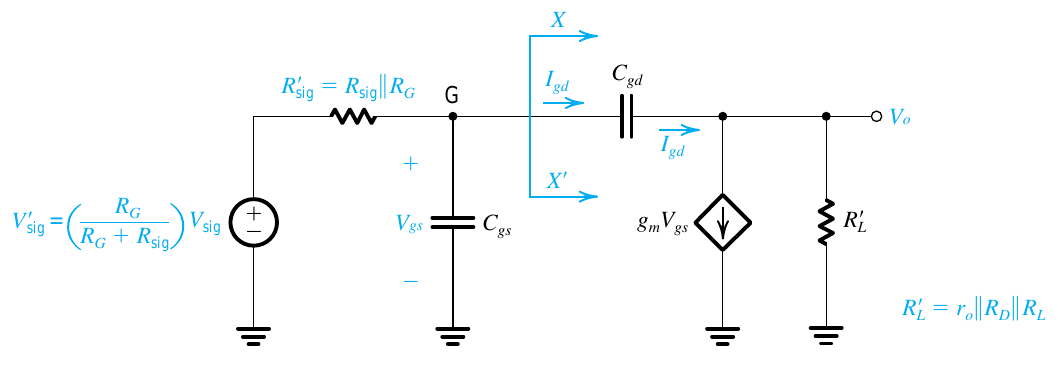
\includegraphics[width=\linewidth]{figures/Problem6443}
    \label{fig:}
  \end{subfigure}%
  \begin{subfigure}{.35\textwidth}
    \centering
    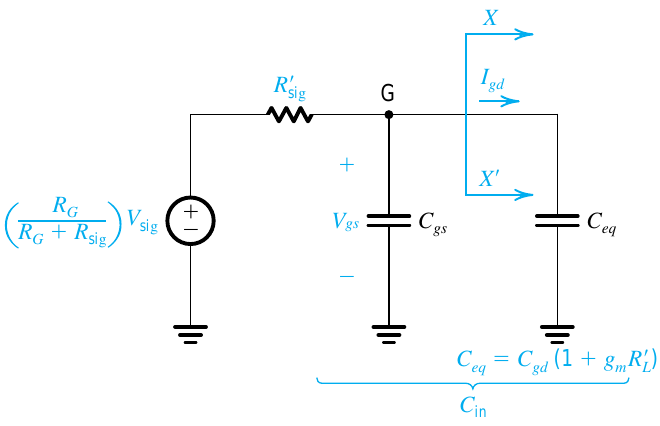
\includegraphics[width=\linewidth]{figures/Problem6444}
    \label{fig:}
  \end{subfigure}
  \label{fig:}
\end{figure}

\begin{equation*}
  \begin{aligned}
    R_G = R_{g1} \parallel R_{g2} = 6 \  \mathrm{k \Omega}
  \end{aligned}
\end{equation*}

\begin{equation*}
  \begin{aligned}
    R_{sig}' = R_{si} \parallel R_G = 0.857 \  \mathrm{k \Omega}
  \end{aligned}
\end{equation*}

\begin{equation*}
  \begin{aligned}
    R_L' = R_d = 4 \  \mathrm{k \Omega}
  \end{aligned}
\end{equation*}

\begin{equation*}
  \begin{aligned}
    C_{eq} = \left( 1 + g_m R_L' \right) C_{gd} = 2.1 \  \mathrm{pF}
  \end{aligned}
\end{equation*}

\begin{equation*}
  \begin{aligned}
    C_{in} = C_{eq} + C_{gs} = 3.1 \  \mathrm{pF}
  \end{aligned}
\end{equation*}

\begin{equation*}
  \begin{aligned}
    f_H = \dfrac{1}{2 \pi R_{sig}' C_{in}} = 60 \  \mathrm{MHz}
  \end{aligned}
\end{equation*}

\begin{equation*}
  \begin{aligned}
    \dot{A}_{vSM} = - g_m R_d \cdot \dfrac{R_G}{R_{si} + R_G} = - 2.74
  \end{aligned}
\end{equation*}




\end{document}